% \documentclass[twocol]{ametsoc}
\documentclass[]{ametsoc}
\usepackage[]{graphicx}
\usepackage{alltt}
\usepackage{siunitx}
%
%==============================================================================
\journal{jcli}

%
%==============================================================================
\bibpunct{(}{)}{;}{a}{}{,}

\title{Effects of Natural Variability of Seawater Temperature, Time Series Length, Decadal Trend and Instrument Precision on the Ability to Detect Temperature Trends}

\authors{Robert Schlegel\correspondingauthor{Robert Schlegel, Department of Biodiversity and Conservation Biology, University of the Western Cape, Bellville, Republic of South Africa.}
 and Albertus Smit}

\affiliation{Department of Biodiversity and Conservation Biology, University of the Western Cape, Bellville, Republic of South Africa}

\email{3503570@myuwc.ac.za}

%
%==============================================================================
\abstract{In South Africa 129 \emph{in situ} temperature time series of up to 43 years are used for investigations of the thermal characteristics of coastal seawater. They are collected with handheld thermometers or underwater temperature recorders (UTRs) and are recorded at precisions from \SIrange{0.5}{0.001}{\degreeCelsius}. Using the natural range of seasonal signals and variability for 84 of these time series, their length, decadal trend and data precision were systematically varied before fitting generalized least squares (GLS) models to study the effect these variables have on trend detection. The variables that contributed most to accurate trend detection in decreasing order were: time series length, decadal trend, variance, percentage of missing data (\%\texttt{NA}) and measurement precision. Time series \textgreater~30 years in length are preferred and though larger decadal trends are modeled more accurately, modeled significance (\emph{p}-value) is largely affected by the variance present. The risk of committing both type 1 and 2 errors increases when $\geq 5\%$\texttt{NA} is present. There is no appreciable effect on model accuracy between measurement precision of \SIrange{0.1}{0.001}{\degreeCelsius} however, measurement precisions of \SI{0.5}{\degreeCelsius} require longer time series to give equally accurate model results. The implication is that the thermometer time series in this dataset, and others around the world, must be at least two years longer than their UTR counterparts to be useful for decadal scale climate change studies. Furthermore, adding older lower precision UTR data to newer higher precision UTR data within the same time series will increase their usefulness for this purpose.}

% 
%==============================================================================
\begin{document}

\maketitle

\section{Introduction}
The roughly 3,000 km of South Africa's coastline is bordered by the Benguela and Agulhas Currents \citep[\emph{e.g.}][]{Roberts2005,Hutchings2009}, which, in combination with other nearshore processes, affect the country's marine coastal ecosystems \citep{Santos2012a}. A thorough understanding of these coastal processes is provided by several physical variables, of which temperature is one of the main determinants \citep[\emph{e.g.}][]{Blanchette2008, Tittensor2010, Couce2012}. The statistical properties of \emph{in situ} seawater temperature time series representing the whole coastline -- such as the annual mean, minimum and maximum temperature, and the thermal range and variance characteristics -- vary greatly among coastal sections due to the varying influence of the Benguela and Agulhas Currents. Based on these thermal properties, the coastline has been classified into a cool temperate west coast, a warm temperate south coast and tending towards sub-tropical along the east coast \citep{Smit2013,Mead2013}. That the ocean temperature of these regions is changing has been reported in recent years. For example, an increase of \SIrange{0.55}{0.7}{\degreeCelsius}~dec$^{-1}$ has been reported in the Agulhas Current \citep{Rouault2009,Rouault2010}, while the southern Benguela has decreased in \SI{0.5}{\degreeCelsius}~dec$^{-1}$ during some parts of the year \citep{Rouault2010}.

The aforementioned climate change trends were derived from remotely-sensed gridded sea surface temperature (SST) products. Whereas newer remotely-sensed gridded SST products are approaching high enough resolutions for use in coastal waters, older longer products that could be used for the detection of long terms trends are not \citep[\emph{e.g.}][]{Chao2009, Qiu2009, Vazquez-Cuervo2013}. A study by \citet{Smit2013} has also shown that remotely-sensed gridded SST data have a warm bias as large as \SI{6}{\degreeCelsius} when compared to coastal \emph{in situ} data. Nevertheless, a widespread approach in coastal ecological research is to use satellite and/or model-generated temperature data as a representation of SST along coastlines \citep[\emph{e.g.}][]{Blanchette2008, Broitman2008a, Tyberghein2012}, because apparently the dangers of applying gridded SSTs to the coast are not widely known or in many places in the world there simply are no suitable \emph{in situ} coastal temperature time series available. It is for this reason that we strongly recommended the use of \emph{in situ} data to support research conducted within 400 m from the shoreline.

Where records of \emph{in situ} coastal seawater temperature do exist, the reliability of many of these datasets that could be used in place of the remotely-sensed SST data remains to be verified. Users of remotely-sensed SST data benefit from it being refined through a number of well documented validation and quality control processes \citep[\emph{e.g.}][]{Reynolds1994, Brown1999, Martin2012}, whereas the standards and methods with which local \emph{in situ} data from a single dataset are collected and refined may differ greatly. For example, there are currently seven organizations and/or governmental departments (hereafter referred to as bodies) contributing coastal seawater temperature data to the South African Coastal Temperature Network (SACTN). These bodies use different methods and instruments to collect their data as no national standard has been set. One consequence of this methodological disparity is that two thirds of the data were sampled with hand-held thermometers that are manually recorded at a data precision of \SI{0.5}{\degreeCelsius}, as opposed to the current generation of underwater temperature recorders (UTRs) with an instrument precision of down to \SI{0.001}{\degreeCelsius}. If these \emph{in situ} temperature data are to be used together \emph{in lieu} of remotely-sensed SST data, it is important that the characteristics of the contributing data sources are understood in terms of their ability to yield useful, reliable and accurate long-term measurements for use in climate change studies.

This prompted us to examine the 129 \emph{in situ} time series that comprise the SACTN. The range of measurement precisions and statistical characteristics of this dataset were used to guide a series of enquiry-driven analyses into the suitability of the time series to yield statistically significant and accurate assessments of decadal temperature change. The length, decadal trend and data precision of each time series were adjusted in a systematic manner, and forms the core of our analyses. Furthermore, the natural variability of each of the time series, which differ more-or-less predictably between coastlines variously affected by the Benguela and Agulhas Currents, was also entered into the analysis. Our aim was to assess the effect that each of these variables has on the ability of a model to produce a robust estimate of time series decadal trend. The effect gaps in the time series may have on the fitting of models was also investigated as many of the time series used here have some missing data scattered throughout, which is unavoidable for a 20+ year time series that is sampled by hand by a single technician at each site.

The study provides a better understanding of some of the determinants of a time series that are influential in the detection success of decadal trends in coastal ocean temperature time series.

\section{Methods}

\subsection{Data Sources}
Our study lies within the political borders of South Africa's coastline and the location of each point of collection may be seen in Figure \ref{figure01}. Of these 129 time series, 43 are recorded with UTRs and the other 86 with hand-held mercury thermometers. The oldest currently running time series began on January 1st, 1972; there are 11 total time series that started in the 70s, 53 more started in the 80s, 34 began in the 90s, 18 in the 00s and 13 in the current decade.

The data are collected using two different methods and a variety of instruments. Hand-held mercury thermometers (which are being phased out in favor of alcohol thermometers or electronic instruments) are used in some instances at the shoreline, and represent seawater temperatures at the surface. At other places, predominantly along the country's east coast, data are collected with glass thermometers from small boats at the location of shark nets along the coast \citep{Cliff1988}. Whereas both types of thermometers allow for a measurement precision of \SI{0.1}{\degreeCelsius}, the recordings are written down at a precision of \SI{0.5}{\degreeCelsius}. Data at other localities are collected using delayed-mode instruments that are permanently moored shallower than 10 m, but generally very close to the surface below the low-water spring tide level.

Over the last 40+ years the electronic instruments used to measure coastal seawater temperatures have changed and improved. The previous standard was the Onset Hobo UTR with a thermal precision of \SI{0.01}{\degreeCelsius}. The new standard currently being phased in is the Starmon Mini UTR. These devices have a maximum thermal precision of \SI[separate-uncertainty = true, multi-part-units = repeat]{0.001(25)}{\degreeCelsius} (http://www.star-oddi.com/). Of the 43 UTR time series in this dataset, 30 were recorded at a precision of \SI{0.001}{\degreeCelsius} for their entirety, five UTR time series include older data that were recorded at a precision of \SI{0.01}{\degreeCelsius} or \SI{0.1}{\degreeCelsius} and so have been rounded down to match this level of precision. Eight additional UTR time series have data recorded at a precision of only \SI{0.1}{\degreeCelsius}.

The thermometer data are recorded manually and saved in an aggregated location at the head offices of the collecting bodies. UTRs are installed and maintained by divers and data are retrieved at least once annually. These data are digital and are downloaded to a hard drive at the respective head offices of the collecting bodies.

\subsection{Data Management}
Each of the seven bodies contributing data to this study have their own method of data formatting. Steps are being taken towards a national standard as we move towards replacing all the thermometer recordings with UTR devices; however, as of the writing of this article, one does not yet exist. Data from each organization were formatted to a project-wide comma-separated values (CSV) format with consistent column headers before any statistical analyses were performed. This allowed for the same methodology to be used across the entire dataset, ensuring consistent analysis. Before analysing the data they were scanned for any values above \SI{35}{\degreeCelsius} or below \SI{0}{\degreeCelsius}. These data points were changed to \texttt{NA}, meaning `not available', before including them in the SACTN dataset.

All analyses and data management performed in this paper were conducted with R version 3.3.1 (2016-06-21) \citep{R}. The script and data used to conduct the analyses and create the figures seen in this paper may be found at https://github.com/schrob040/Trend\_Analysis.

Any time series with a temporal precision greater than one day were averaged into daily values before being aggregated into the SACTN. A series of additional checks were then performed (\emph{e.g.} removing long stretches in the time series without associated temperature recordings) and time series shorter than five calendar years, collected at depths greater than 10 m or missing more than 15\% of their monthly values were removed. At the time of this analysis, this usable daily dataset consisted of 84 time series, consisting of 819,499 days of data; these data were then binned further to the 26,924 monthly temperature values available for use in this study.

\subsection{Systematic Analysis of Time Series}
We used the 84 time series simply for their variance properties (comprised of seasonal, interannual, decadal and ‘noise’ components), which reflect that of the thermal environment naturally present along the roughly 3,000 km of South African coastline. Linear trends that may have been present in each time series were removed prior to the ensuing analysis by applying an ordinary least squares regression and keeping the detrended residuals as anomaly time series. In doing so we avoided the need to simulate a series of synthetic time series, whose variance components may not have been fully representative of that naturally present in coastal waters. These detrended anomaly time series (henceforth simply called `time series') represent a range of time scales from 72 to 519 months in duration.

To each of the 84 time series we artificially added linear decadal trends of \SIrange{0.00}{0.20}{\degreeCelsius}~dec$^{-1}$. In other words, we now had time series that captured the natural thermal variabilities around the coast, but with their decadal trends known \emph{a priori}. The range of decadal trends was selected based around the global average of \SI{0.124}{\degreeCelsius} from \citet{Kennedy2011} and used in \citet{IPCC2013}. Furthermore, in order to represent the instrumental precision of the instruments used to collect these time series, we rounded each of these (84 time series $\times~5$ decadal trends) to four levels of precision: \SI{0.5}{\degreeCelsius}, \SI{0.1}{\degreeCelsius}, \SI{0.01}{\degreeCelsius} and \SI{0.001}{\degreeCelsius}. Consequently, we had a pool of 1,680 time series with which to work.

To gain further insight into the effect of time series length on trend detection, each time series was first shortened to a minimum length of 5 years, starting in January so that the timing of the seasonal signal for each time series would be equitable. After fitting the model (see \emph{Time Series Model}, below) to all 1,680 of the shortened time series, the next year of data for each time series was added and the models fitted again. This process was iterated until the full length of each time series was attained. For example, if a time series consisted of 12 full years of data, it would require 160 models (8 iterations of increasing length $\times~5$ decadal trends $\times~4$ levels of precision); similarly, 720 models would be applied to a 40 year time series. Considering the 84 time series available, the total number of individual models required to capture each combination of variables quickly increased to 36,220.

Our approach of fitting models to each of the semi-artificial time series that we generated allowed us to study the effect that the relevant variables (time series length, natural variability, added slope and level of measurement precision) has on the ability of the time series model to faithfully detect the decadal thermal trend, which was known \emph{a priori}. The primary results of interest in these analyses were the significance (\emph{p}-value) of the model fit, the accuracy of the decadal trend determined by the GLS model as well as the error associated with the trend estimate.

\subsection{Time Series Model}
The selection of the appropriate model can greatly influence the ability to detect trends \citep{Franzke2012}. Two broad approaches are widely used in climate change research \citep{IPCC2013}. The first group of models estimates linear trends, and although linearity may not reflect reality (\emph{i.e.} trends are very frequently non-linear), these models do provide the convenience of producing an easy to understand decadal trend \citep[\emph{e.g.} \SI{0.106}{\degreeCelsius}~dec$^{-1}$;][]{Wilks2011,IPCC2013}. The other group accommodates non-linear trajectories of temperature through time by the use of higher-degree polynomial terms or non-parametric smoothing splines, but the inconvenience comes from not being able to easily compare models among sites \citep{Wood2006,Scinocca2010}. Both groups of models can accommodate serially correlated residuals, which is often the cause for much criticism due to their effect on the uncertainty of the trend estimates \citep{vonStorch1999,Santer2008}. For example, Generalized Least Squares (GLS; yielding estimates of linear trends) and Generalized Additive Mixed Models (GAMM; non-linear fitting with no trend estimate provided) can both capture various degrees of serial autocorrelation \citep{pinheiro2006mixed,Wood2006}. Although our exploratory analysis assessed two parametrizations of each of the model groups, we opted to proceed here with a GLS equipped with a second-order autoregressive AR(2) correlation structure fitted using Restricted Maximum Likelihood \citep[REML;][]{pinheiro2006mixed}:

$$y_{t} = \beta_{0} + \beta_{1}x_{t} + \epsilon_{t}$$

where the lag-2 autocorrelated residuals are given by

$$\epsilon_{t} = \phi_{1}\epsilon_{t-1} + \phi_{2}\epsilon_{t-2} + w_{t}$$

and the white noise series is

$$w_{t} \sim \mathrm{i.i.d.}~N(0,\sigma^{2})$$

This is similar to that of the IPCC, although the latter uses an AR(1) error term \citep{IPCC2013supp}. Another difference from the IPCC approach is that we nested the autoregressive component within year. This modelling approach allowed us to assess how various properties of the detrended data sets would affect the models' ability to detect trends -- in other words, by comparing the estimates of the trends themselves and how these deviate from the known trend.

\section{Results}
The residuals for the base 84 detrended time series may be seen in Figure \ref{figure02}. From these detrended time series the length, decadal trend and precision variables were systematically manipulated as explained in the methods. It was found that the important variables affecting the accuracy of the slope detected by the GLS model, in decreasing order, were: i) time series length; ii) the size of the added decadal trend; iii) initial SD of the time series (after detrending but prior to adding artificial slopes); iv) the amount of \texttt{NA}; and iv) measurement precision. These variables influence the model fits in a systematic manner.

As would be expected, the size of the decadal trend estimated by the GLS increases in direct proportion to the decadal trend which we added and therefore knew \emph{a priori}. What is especially noteworthy in this analysis is that time series of longer duration more often result in trend estimates converging with the actual trend than those of shorter length (Figure \ref{figure03}). This effect is most evident from around 30 years. Furthermore, how well the estimated model trend converges with the actual trend is also very visible in the standard error (SE) of the trend estimate (Figure \ref{figure04}): models fitted to short time series always have modeled trends with larger SE compared to longer ones. The strength of this correlation is \emph{r}~=~0.56 (\emph{p}~\textless~0.001) and it remains virtually unchanged as the added decadal trend increases. The \emph{p}-value of the fitted models also vary in relation to time series duration and to the steepness of the added decadal trend (Figure \ref{figure05}). It is usually the longer time series equipped with steeper decadal trends that are able to produce model fits with estimated trends that are statistically significant. Note, however, that this \emph{p}-value tests the null hypothesis that the estimated trend is no different from \SI{0}{\degreeCelsius}~dec$^{-1}$ at \emph{p} $\leq 0.05$, and \emph{not} that the slope is not different from the added trend. Taken together, these outcomes show that although our GLS model can very often result in trend estimates that \emph{approach} the true trend, it is seldom that those estimates are statistically significant in the sense that the estimated trends differ statistically from \SI{0}{\degreeCelsius}~dec$^{-1}$.

The variance of the detrended data is another variable that can affect model fitting, but its only systematic influence concerns the SE of the trend estimate. Here, it acts in a manner that is entirely consistent across all \emph{a priori} trends (Figure \ref{figure06}). What we see is that as the variance of the data increases (represented here as standard deviation, SD) the SE of the slope estimates increases too. Moreover, it does so disproportionately more for time series of shorter duration. Again, as we have seen with the estimated trend that converges to the true trend around 30 years, so too does the initial SD of the data cease to be important in time series of around 3 decades in length.

The number of \texttt{NA}s permitted in any of our time series was limited to 15\% per time series. Twenty-five of the 84 time series have fewer than 1\% \texttt{NA}. An additional 45 time series have up to 5\% \texttt{NA}, 10 have up to 10\% \texttt{NA} and 4 have up to 15\% \texttt{NA}. The mean number of \texttt{NA} for the data is 2.65\%. The relationship between \%\texttt{NA} and the \emph{p}-value of the models is shown in Figure \ref{figure07}. At 2.5\% or fewer \texttt{NA} their presence does not have any discernible effect on resultant \emph{p}-values. Progressively increasing the number of \texttt{NA}s above 5\%, however, leads to a drastic improvement of models fitted to series with no or gently increasing decadal trends (these generally have very large \emph{p}-values indicative of very poor fits, perhaps due to the presence of a very weak signal), and a significant deterioration of models fitted to data with steep decadal trends (for these data, the model generally fits better at low numbers of \texttt{NA}s, as suggested by the greater number of \emph{p}-values that approach 0.05). In other words, the inclusion of missing values results in time series with no added decadal trend to veer away from \SI{0}{\degreeCelsius}~dec$^{-1}$ towards a situation where they may erroneously appear to display a trend. On the other hand, time series that do indeed have decadal trends tend to produce fits that are not significantly different from \SI{0}{\degreeCelsius}~dec$^{-1}$.

Regarding the effect that the level of measurement precision has on the GLS models, we see in Figure \ref{figure08} that decreasing the precision from \SI{0.001}{\degreeCelsius} to \SI{0.01}{\degreeCelsius} has an undetectable effect on any differences in the modeled trends. The Root Mean Square Error (RMSE) between the slopes estimated from \SI{0.001}{\degreeCelsius} and \SI{0.01}{\degreeCelsius} data is 0.001. The correspondence between the slopes estimated for data reported at \SI{0.5}{\degreeCelsius} compared to that at \SI{0.001}{\degreeCelsius} decreases to a RMSE of 0.03.

The effect of decreasing data measurement precision from \SI{0.001}{\degreeCelsius} to \SI{0.5}{\degreeCelsius} has almost no appreciable effect on any of the measures of variance presented in this study. The effect of measurement precision on the accuracy of the modeled slope, however, becomes very pronounced going from \SI{0.1}{\degreeCelsius} to \SI{0.5}{\degreeCelsius}. This effect is larger on smaller decadal trends. For example, at a trend of \SI{0.05}{\degreeCelsius}~dec$^{-1}$, the deviation from the true value of models fitted to data with a precision of \SI{0.1}{\degreeCelsius} is negligible; however, the accuracy of the fitted model on data recorded at a precision of \SI{0.5}{\degreeCelsius} with a real trend of \SI{0.05}{\degreeCelsius}~dec$^{-1}$ is 10.81\% different on average (\emph{i.e.} given a slope of \SI{0.05}{\degreeCelsius}~dec$^{-1}$ the model detects slopes of \SI{0.055}{\degreeCelsius}~dec$^{-1}$). This accuracy of the models improves to an average difference of 6.44\% with a slope of \SI{0.10}{\degreeCelsius}~dec$^{-1}$, 2.24\% at \SI{0.15}{\degreeCelsius}~dec$^{-1}$ and decreases slightly to 2.30\% at \SI{0.20}{\degreeCelsius}~dec$^{-1}$. A precision of \SI{0.5}{\degreeCelsius} always provides clearly less accurate modeled trends than at higher precisions; however, the current analysis did not highlight one precision that consistently provides the most accurate estimate of the trends. This may however become determinable in an analysis of synthetic data with variance structures that are manipulated in a more consistent manner.

As the actual time series used to generate the data for this study are predominantly greater than 300 months in length and recorded at a data precision of \SI{0.5}{\degreeCelsius}, we would be remiss not to investigate the interaction between the increase in accuracy provided by a lengthy time series, against the decrease caused by a data precision of \SI{0.5}{\degreeCelsius}. In other words, at what point does a model fitted to a longer time series, with less precise measurements (\emph{e.g.} those taken by thermometers and reported at a precision of \SI{0.5}{\degreeCelsius}), become as accurate as a time series with more precise measurements (\emph{e.g.} UTRs)? Figure \ref{figure08} shows how varied the modeled trends become when a precision of \SI{0.5}{\degreeCelsius} is used, and we see here that when these low resolution time series have a shallow slope of \SI{0.05}{\degreeCelsius}~dec$^{-1}$, a fitted model requires 24 months of additional data on average to have a comparable level of accuracy to a model fitted to data recorded at a precision of \SI{0.1}{\degreeCelsius}. This difference in length decreases to 16 months when a larger slope \SI{0.20}{\degreeCelsius}~dec$^{-1}$ is used.

An analysis with a large number of variables as shown here is bound to have a medley of complex interactions between the various statistics being measured; however, much of the range seen in the results of the GLS models can be well explained by the influence of one independent variable, or two operating in concert, as we have shown above. The most important of these variables has clearly been length.

\section{Discussion}
The strongest finding of this analysis is that the accurate detection of long-term trends in time series primarily concerns the length of a dataset. But there is also a host of nuances resulting from time series length, the steepness of the decadal trend the model is asked to detect, the influence of the SD of a time series, the amount of missing values and the precision at which the data have been measured or recorded that interact with one-another and which must be considered.

Whereas time series with smaller variances (shown as SD in this study) generally produce model fits that are statistically significant (\emph{i.e.} with decadal trends that are significantly different from \SI{0}{\degreeCelsius}~dec$^{-1}$ at \emph{p} \textless~0.05) and with smaller SE of the estimated trends after shorter lengths of time, we also see that increasing a time series' length beyond 25 years, but preferably beyond 30 years, will increase the likelihood of detecting a decadal temperature change even in very variable data sets. Detecting temperature change in highly variable coastal environments, such as those around the coast of South Africa and many temperate coastal environments globally, will therefore benefit from access to the longest possible time series available. This phenomenon is demonstrated in Figure \ref{figure05}, which uses color to show the time series binned by the three different coastal sections of South Africa \citep{Smit2013}. Of these three coastal sections the east coast is known to have the most stable thermal regime (\emph{i.e.} with the smallest variance), with the south coast having the greatest variance. Long time series at sites of low variance result in great improvements in our ability to detect significant climate change trends, and this effect is most obvious in time series with steeper decadal trends. The selection of sites for long-term monitoring must therefore account for the location of study and necessitate adequate planning to collect a long enough time series.

The detection of long-term trends require long-term data, a fact that is already firmly established in climate change research \citep{Ohring2005, IPCC2013}. The length of these time series is firmly under the control of the investigator with sufficient foresight and perseverance to plan the installation and management of new instrument networks that will yield usable results only after about three-quarters of a typical academic career has passed. Should such data already exist -- and considering the scarcity of such long-term records that are already yielding benefits today -- we must ensure that these sources of data are managed and curated with great care and diligence as they are practically irreplaceable. For this reason, it is essential that we understand the inherent strengths and weaknesses of such existing sources of data so that we may fully maximize their utility and extract from them the model coefficients needed to detect decadal temperature trends, and know the accuracy of these estimates to the best of our ability. There are many time series \textless~20 years in length that should be avoided, where possible, for trend analysis. These will mature with time and their maintenance need to be ensured going forward.

Aside from length, the most powerful time series have measurements that are taken regularly. The inclusion of too many missing values (\texttt{NA}s) in the data sets must be avoided. We have shown that permitting 5\% \texttt{NA}s or more into our time series has a drastic and significant influence on the chance of committing a type 1 error (arriving at `false positive,' \emph{i.e.} detecting a trend when none exists) for time series with no or very gentle decadal trends. On the other hand, the inclusion of \texttt{NA}s in data sets with a decadal trend present tends to cause an increase in the probability of committing a type 2 error (\emph{i.e.} finding `false negatives'). Although our modern UTR data sets generally have fewer \texttt{NA}s than we should be concerned about -- therefore with a low chance of committing type 1 or type 2 errors -- the presence of \texttt{NA}s may seriously compromise some of the time series that are still being collected by hand using hand-held thermometers.

We have demonstrated clearly that as the steepness of an expected decadal trend increases, the ability for it to be modeled accurately increases, too. Our GLS model is generally not able to detect trends that are significantly different from \SI{0}{\degreeCelsius}~dec$^{-1}$ unless a slope of \SI{0.20}{\degreeCelsius}~dec$^{-1}$ exists. Very rarely were we able to produce significant model fits at shallower slopes. Finding significant trends at \textless~\SI{0.05}{\degreeCelsius}~dec$^{-1}$ was not possible. Based on the relationship between SD and the added decadal trend, we see that time series with a SD of \SI{1.5}{\degreeCelsius} (the bulk of the time series here) and a decadal trend of \SI{0.10}{\degreeCelsius}~dec$^{-1}$ should consist of roughly 640 months of data before our GLS model would regularly be able to detect a significant trend (\emph{p} \textless~0.05). This finding is somewhat discouraging as most global analyses of decadal SST change based on gridded SST products estimate a trend closer to \SI{0.1}{\degreeCelsius}~dec$^{-1}$ \citep[\emph{e.g.}][]{IPCC2013}. This means that the trends present in most time series representative of very variable coastal environments that exhibit the same variance structure as that of our data are probably unlikely to be detected as significant, even if they do indeed exist. In other words, the chance of committing a type 2 error is probably very real for such systems, unless time series \textgreater~50 years are available.

As 50 year coastal seawater temperature time series are probably very scarce, it is important to note that those measured at precisions of \SIrange{0.1}{0.001}{\degreeCelsius} require fewer months of data to detect long term trends. Based on the data presented here, we calculated that time series measured at a low precision (\SI{0.5}{\degreeCelsius}) may require as much as an additional 24 months of data to accurately detect long-term trends. One of the motivators for this paper was to investigate the effect measurement precision has on a time series' ability to produce results useful for investigations of long-term climate change, and to validate the use of the low precision \SI{0.5}{\degreeCelsius} thermometer data. This is an important consideration as many studies investigating the effects of climate change \citep[\emph{e.g.}][]{Grant2010, Scherrer2010, Lathlean2012} do use lower precision \SI{0.1}{\degreeCelsius} data. Whereas the precision of much of our data is below the current standard of \SI{0.1}{\degreeCelsius} required for climate change research \citep{Ohring2005,Jarraud2008}, the length of the thermometer time series makes them a valuable asset. The average length of the thermometer time series in the SACTN, from which the 84 time series used in this study were drawn, is 349 months. The average length of the UTR time series is 167 months. Given this difference in the lengths of the time series, even after correcting for the negative effect of low measurement precision, the time series collected with thermometers are currently more useful for climate change research than the UTR time series within the SACTN. Because time series with data precisions of \SIrange{0.1}{0.001}{\degreeCelsius} produce comparable results, newer higher precision UTR data may be combined with older lower precision UTR data within the same time series without concern that the reduced overall data precision may have a negative impact on a model's ability to detect decadal trends. Extending time series in this way will serve to make them more dependable as length is the primary criterion through which one should initially assess a time series ability to suggest the presence of climate change before refining ones assumptions with any statistical analyses. A time series with data precision greater than \SI{0.1}{\degreeCelsius} is therefore only necessary when an investigation requires that the decadal trend be known to an accuracy of \SI{0.01}{\degreeCelsius} or greater \citep[\emph{e.g.}][]{Karl2015}.

It is important to take note of the accuracy of the models, not only to focus on the significance of their results. Indeed, the \emph{p}-value given for the slope in a model does not show how well the model detects the true trend in the data (known \emph{a-priori} in this study); rather, it tells us if the detected trend is significantly different from \SI{0}{\degreeCelsius}~dec$^{-1}$. This is not particularly useful for applying the results of climate change research more broadly to biotic interests. For example, of the 1344 models (84 base time series $\times~4$ decadal trends $\times~4$ levels of precision) fitted to time series with decadal trends $\geq~\SI{0.05}{\degreeCelsius}$~dec$^{-1}$, 317 of these  were accurate to within 10\% of the decadal trend known \emph{a priori}, but not significant (\emph{p}~$\geq~0.05$). That a long term trend does exist, may be accurately detected by a model and related to an observed change in the natural world -- such as range expansion/contraction of coastal biota \citep{Bolton2012,Straub2016,Wernberg2016} -- is more important than whether or not the model can show if that trend is significantly different from \SI{0}{\degreeCelsius}~dec$^{-1}$ in a statistical sense.

We must mention also that much of the meta-data pertaining to the older temperature records used here have over time been lost. As with the bulk of the International Comprehensive Ocean-Atmosphere Data Set \citep[ICOADS;][]{Freeman:2016db}, \emph{in situ} coastal seawater temperature monitoring that started in the 1970s in South Africa was not developed with climate change research in mind, and comprehensive records that keep track of details of the instruments used, calibration, their turnover, change in monitoring methods and locations and so forth are not always available as per modern requirements \citep{Aguilar2003}. For studies of climate change \emph{per se} this is a serious limitation and it prevents us from knowing anything about the accuracy of the instruments or potential issues of drift (stability) that may have occurred. We do know however that all time series sampled with thermometers were sampled only with thermometers, and \emph{vice versa} for the UTR time series, ensuring that the precisions of the measured data used in this study are correct. Moving forward with the further development of the SACTN and the establishment of a national standard of data collection and instrument maintenance, we are able to record and archive all these levels of pertinent meta-data, and allowing for the enforcement of SI traceability and the accurate measurement of instrument drift \citep{Jarraud2008}. Nevertheless, the detrended anomaly time series used here were taken only for their variance properties, which we think accurately reflect that of the various coastal sections around the coast. They provide a strong backbone for semi-artificial time series, and we have shown how important insights about model fitting could be derived from these data.

\section{Conclusion}
We draw several key conclusions:

\begin{enumerate}
\item There is a rapid increase in the accuracy and significance of modeled trends as time series lengths extend from 10 to 20 years. This improvement slows from 20 to 30 years, and as time series approach 40 years in length the accuracy of models becomes nearly exact. Modelled trends from time series at or under 25 years in length should be interpreted with extreme caution.

\item For our variable coastal seawater, a time series of 520 months in length is required to detect a decadal trend in line with the global average (\emph{i.e.} near \SI{0.1}{\degreeCelsius}~dec$^{-1}$) with perfect accuracy; however, an additional 120 months of data is often required for the detected trend to be considered significant (\emph{p} $\leq 0.05$).

\item The length of a time series required to detect a decadal trend at \SI{0.1}{\degreeCelsius}~dec$^{-1}$ may rapidly exceed 100 years when a large amount of variance is present.

\item The larger the decadal trend within a time series, the more accurately it will be modeled regardless of the amount of variance in the time series.

\item There is a complicated relationship between the accuracy of a trend fitted to a time series and the \%\texttt{NA} of that time series. As the \%\texttt{NA} increases, so too does the chance of committing type 1 (with gentle trends) or type 2 errors (with steeper trends).

\item A measurement precision greater than \SI{0.5}{\degreeCelsius} is not required to confidently detect the long-term trend in a time series; however, precisions at or greater than \SI{0.1}{\degreeCelsius} may reduce the length of time required to accurately detect a long term trend, if one does exist, by as much as two years.

\item Improving the precision of measurements to greater than \SI{0.1}{\degreeCelsius} has almost no appreciable effect on a models ability to detect a long-term trend, provided that the reported effect size matches the level of precision by the instruments.
\end{enumerate}

We understand that time series of \textgreater 30 years may be exceedingly rare. Therefore, as we move forward as a scientific community investigating the issues of climate change, the continuity of any current time series of sufficient length must be ensured as these commodities are practically irreplaceable.
%
%==============================================================================

\acknowledgments
The authors would like to thank DAFF, DEA, EKZNW, KZNSB, SAWS and SAEON for their contributions of the raw data used in this study. Without it, this article and the SACTN would not be possible. This research was supported by NRF Grant (CPRR14072378735). The authors report no financial conflicts of interests.

%
%==============================================================================

% \bibliographystyle{ametsoc2014}
% \bibliography{trends}

% %
% %==============================================================================
\begin{thebibliography}{41}
\providecommand{\natexlab}[1]{#1}
\providecommand{\url}[1]{\texttt{#1}}
\renewcommand{\UrlFont}{\rmfamily}
\providecommand{\urlprefix}{URL }
\expandafter\ifx\csname urlstyle\endcsname\relax
  \providecommand{\doi}[1]{doi:\discretionary{}{}{}#1}\else
  \providecommand{\doi}{doi:\discretionary{}{}{}\begingroup
  \urlstyle{rm}\Url}\fi
\providecommand{\eprint}[2][]{\url{#2}}

\bibitem[{Aguilar et~al.(2003)Aguilar, Auer, Brunet, Peterson,, and
  Wieringa}]{Aguilar2003}
Aguilar, E., I.~Auer, M.~Brunet, T.~Peterson, and J.~Wieringa, 2003: Guidelines
  on climate metadata and homogenization, wmo-td no. 1186 (wcdmp2).
  \textit{World Meteorological Organization, Geneva}.

\bibitem[{Blanchette et~al.(2008)Blanchette, {Melissa Miner}, Raimondi, Lohse,
  Heady,, and Broitman}]{Blanchette2008}
Blanchette, C.~A., C.~{Melissa Miner}, P.~T. Raimondi, D.~Lohse, K.~E.~K.
  Heady, and B.~R. Broitman, 2008: {Biogeographical patterns of rocky
  intertidal communities along the Pacific coast of North America}.
  \textit{Journal of Biogeography}, \textbf{35~(9)}, 1593--1607.

\bibitem[{Bolton et~al.(2012)Bolton, Anderson, Smit,, and Rothman}]{Bolton2012}
Bolton, J.~J., R.~J. Anderson, A.~J. Smit, and M.~D. Rothman, 2012: {South
  African kelp moving eastwards: the discovery of Ecklonia maxima (Osbeck)
  Papenfuss at De Hoop Nature Reserve on the south coast of South Africa}.
  \textit{African Journal of Marine Science}, \textbf{34~(1)}, 147--151.

\bibitem[{Broitman et~al.(2008)Broitman, Mieszkowska, Helmuth,, and
  Blanchette}]{Broitman2008a}
Broitman, B.~R., N.~Mieszkowska, B.~Helmuth, and C.~A. Blanchette, 2008:
  {Climate and recruitment of rocky shore intertidal invertebrates in the
  eastern North Atlantic.} \textit{Ecology}, \textbf{89~(11 Suppl)}, S81--90.

\bibitem[{Brown et~al.(1999)Brown, Minnett, Evans, Kearns, Kilpatrick, Kumar,
  Sikorski,, and Z{\'{a}}vody}]{Brown1999}
Brown, O.~B., P.~J. Minnett, R.~Evans, E.~Kearns, K.~Kilpatrick, A.~Kumar,
  R.~Sikorski, and A.~Z{\'{a}}vody, 1999: {MODIS Infrared Sea Surface
  Temperature Algorithm Algorithm Theoretical Basis Document Version 2.0}.
  \textit{University of Miami}, 31\,098--33\,149.

\bibitem[{Chao et~al.(2009)Chao, Li, Farrara,, and Hung}]{Chao2009}
Chao, Y., Z.~Li, J.~D. Farrara, and P.~Hung, 2009: {Blending sea surface
  temperatures from multiple satellites and in situ observations for coastal
  oceans}. \textit{Journal of Atmospheric and Oceanic Technology},
  \textbf{26~(7)}, 1415--1426, \doi{10.1175/2009JTECHO592.1}.

\bibitem[{Cliff et~al.(1988)Cliff, Dudley,, and Davis}]{Cliff1988}
Cliff, G., S.~F.~J. Dudley, and B.~Davis, 1988: {Sharks caught in the
  protective gill nets off Natal, South Africa. 1. The sandbar shark
  Carcharhinus plumbeus (Nardo)}. \textit{South African Journal of Marine
  Science}, \textbf{7~(1)}, 255--265.

\bibitem[{Couce et~al.(2012)Couce, Ridgwell,, and Hendy}]{Couce2012}
Couce, E., A.~Ridgwell, and E.~J. Hendy, 2012: {Environmental controls on the
  global distribution of shallow-water coral reefs}. \textit{Journal of
  Biogeography}, \textbf{39~(8)}, 1508--1523.

\bibitem[{Franzke(2012)}]{Franzke2012}
Franzke, C., 2012: {Nonlinear trends, long-range dependence, and climate noise
  properties of surface temperature}. \textit{Journal of Climate},
  \textbf{25~(12)}, 4172--4183, \doi{10.1175/JCLI-D-11-00293.1}.

\bibitem[{Freeman et~al.(2016)}]{Freeman:2016db}
Freeman, E., and Coauthors, 2016: {ICOADS release 3.0: a major update to the
  historical marine climate record}. \textit{International Journal of
  Climatology}, 1--22.

\bibitem[{Grant et~al.(2010)Grant, Tronina, Ramalho, {Kurz Besson},
  Lobo-Do-Vale, {Santos Pereira}, Jones,, and Chaves}]{Grant2010}
Grant, O.~M., L.~Tronina, J.~C. Ramalho, C.~{Kurz Besson}, R.~Lobo-Do-Vale,
  J.~{Santos Pereira}, H.~G. Jones, and M.~M. Chaves, 2010: {The impact of
  drought on leaf physiology of Quercus suber L. trees: Comparison of an
  extreme drought event with chronic rainfall reduction}. \textit{Journal of
  Experimental Botany}, \textbf{61~(15)}, 4361--4371, \doi{10.1093/jxb/erq239}.

\bibitem[{Hartmann et~al.(2013)}]{IPCC2013supp}
Hartmann, D., and Coauthors, 2013: Observations: Atmosphere and surface
  supplementary material. in: Climate change 2013: The physical science basis.

\bibitem[{Hutchings et~al.(2009)}]{Hutchings2009}
Hutchings, L., and Coauthors, 2009: {The Benguela Current: An ecosystem of four
  components}. \textit{Progress in Oceanography}, \textbf{83~(1-4)}, 15--32,
  \doi{10.1016/j.pocean.2009.07.046}.

\bibitem[{Jarraud(2008)}]{Jarraud2008}
Jarraud, M., 2008: Guide to meteorological instruments and methods of
  observation (wmo-no. 8). \textit{World Meteorological Organisation, Geneva}.

\bibitem[{Karl et~al.(2015)}]{Karl2015}
Karl, T.~R., and Coauthors, 2015: {Possible artifacts of data biases in the
  recent global surface warming hiatus}. \textit{Science}, \textbf{348~(6242)},
  1469--1472, \doi{10.1126/science.aaa5632}.

\bibitem[{Kennedy et~al.(2011)Kennedy, Rayner, Smith, Saunby,, and
  Parker}]{Kennedy2011}
Kennedy, J.~J., N.~A. Rayner, R.~O. Smith, M.~Saunby, and D.~E. Parker, 2011:
  {Reassessing biases and other uncertainties in sea-surface temperature
  observations measured \emph{in situ} since 1850, Part 1: measurement and
  sampling uncertainties}. \textit{Journal of Geophysical Research
  Atmospheres}, \textbf{116}.

\bibitem[{Lathlean and Minchinton(2012)Lathlean, and Minchinton}]{Lathlean2012}
Lathlean, J.~A., and T.~E. Minchinton, 2012: {Manipulating thermal stress on
  rocky shores to predict patterns of recruitment of marine invertebrates under
  a changing climate}. \textit{Marine Ecology Progress Series}, \textbf{467},
  121--136, \doi{10.3354/meps09996}.

\bibitem[{Martin et~al.(2012)}]{Martin2012}
Martin, M., and Coauthors, 2012: {Group for High Resolution Sea Surface
  temperature (GHRSST) analysis fields inter-comparisons. Part 1: A GHRSST
  multi-product ensemble (GMPE)}. \textit{Deep Sea Research Part II: Topical
  Studies in Oceanography}, \textbf{77-80}, 21--30.

\bibitem[{Mead et~al.(2013)}]{Mead2013}
Mead, A., and Coauthors, 2013: {Human-mediated drivers of change {\textemdash}
  impacts on coastal ecosystems and marine biota of South Africa}.
  \textit{African Journal of Marine Science}, \textbf{35~(3)}, 403--425.

\bibitem[{Ohring et~al.(2005)Ohring, Wielicki, Spencer, Emery,, and
  Datla}]{Ohring2005}
Ohring, G., B.~Wielicki, R.~Spencer, B.~Emery, and R.~Datla, 2005: {Satellite
  instrument calibration for measuring global climate change: report of a
  workshop}. \textit{Bulletin of the American Meteorological Society},
  \textbf{86~(9)}, 1303--1313.

\bibitem[{Pinheiro and Bates(2006)Pinheiro, and Bates}]{pinheiro2006mixed}
Pinheiro, J., and D.~Bates, 2006: \textit{Mixed-effects models in S and
  S-PLUS}. Springer Science \& Business Media.

\bibitem[{Qiu et~al.(2009)Qiu, Wang, Kawamura, Guan,, and Qin}]{Qiu2009}
Qiu, C., D.~Wang, H.~Kawamura, L.~Guan, and H.~Qin, 2009: {Validation of AVHRR
  and TMI-derived sea surface temperature in the northern South China Sea}.
  \textit{Continental Shelf Research}, \textbf{29~(20)}, 2358--2366.

\bibitem[{{R Core Team}(2013)}]{R}
{R Core Team}, 2013: \textit{{R: A Language and Environment for Statistical
  Computing}}. Vienna, Austria, R Foundation for Statistical Computing,
  \urlprefix\url{http://www.r-project.org/}.

\bibitem[{Reynolds and Smith(1994)Reynolds, and Smith}]{Reynolds1994}
Reynolds, R.~W., and T.~M. Smith, 1994: {Improved Global Sea Surface
  Temperature Analyses Using Optimum Interpolation}. \textit{Journal of
  Climate}, \textbf{7~(6)}, 929--948.

\bibitem[{Roberts(2005)}]{Roberts2005}
Roberts, M.~J., 2005: {Chokka squid (Loligo vulgaris reynaudii) abundance
  linked to changes in South Africa's Agulhas Bank ecosystem during spawning
  and the early life cycle}. \textit{ICES Journal of Marine Science},
  \textbf{62~(1)}, 33--55, \doi{10.1016/j.icesjms.2004.10.002}.

\bibitem[{Rouault et~al.(2009)Rouault, Penven,, and Pohl}]{Rouault2009}
Rouault, M., P.~Penven, and B.~Pohl, 2009: {Warming in the Agulhas Current
  system since the 1980's}. \textit{Geophysical Research Letters},
  \textbf{36~(12)}, 1--5.

\bibitem[{Rouault et~al.(2010)Rouault, Pohl,, and Penven}]{Rouault2010}
Rouault, M., B.~Pohl, and P.~Penven, 2010: {Coastal oceanic climate change and
  variability from 1982 to 2009 around South Africa}. \textit{African Journal
  of Marine Science}, \textbf{32~(2)}, 237--246.

\bibitem[{Santer et~al.(2008)}]{Santer2008}
Santer, B.~D., and Coauthors, 2008: Consistency of modelled and observed
  temperature trends in the tropical troposphere. \textit{International Journal
  of Climatology}, \textbf{28~(13)}, 1703--1722.

\bibitem[{Santos et~al.(2012)Santos, Gomez-Gesteira, DeCastro,, and
  Alvarez}]{Santos2012a}
Santos, F., M.~Gomez-Gesteira, M.~DeCastro, and I.~Alvarez, 2012: {Differences
  in coastal and oceanic SST trends due to the strengthening of coastal
  upwelling along the Benguela current system}. \textit{Continental Shelf
  Research}, \textbf{34}, 79--86.

\bibitem[{Scherrer and K{\"{o}}rner(2010)Scherrer, and
  K{\"{o}}rner}]{Scherrer2010}
Scherrer, D., and C.~K{\"{o}}rner, 2010: {Infra-red thermometry of alpine
  landscapes challenges climatic warming projections}. \textit{Global Change
  Biology}, \textbf{16~(9)}, 2602--2613,
  \doi{10.1111/j.1365-2486.2009.02122.x}.

\bibitem[{Scinocca et~al.(2010)Scinocca, Stephenson, Bailey, Austin
  et~al.}]{Scinocca2010}
Scinocca, J., D.~B. Stephenson, T.~C. Bailey, J.~Austin, and Coauthors, 2010:
  Estimates of past and future ozone trends from multimodel simulations using a
  flexible smoothing spline methodology. \textit{Journal of Geophysical
  Research: Atmospheres}, \textbf{115~(D3)}.

\bibitem[{Smit et~al.(2013)Smit, Roberts, Anderson, Dufois, Dudley, Bornman,
  Olbers,, and Bolton}]{Smit2013}
Smit, A.~J., M.~Roberts, R.~J. Anderson, F.~Dufois, S.~F.~J. Dudley, T.~G.
  Bornman, J.~Olbers, and J.~J. Bolton, 2013: {A coastal seawater temperature
  dataset for biogeographical studies: Large biases between in situ and
  remotely-sensed data sets around the coast of South Africa}. \textit{PLoS
  ONE}, \textbf{8~(12)}, \doi{10.1371/journal.pone.0081944}.

\bibitem[{Stocker et~al.(2013)}]{IPCC2013}
Stocker, T., and Coauthors, 2013: \textit{IPCC, 2013: climate change 2013: the
  physical science basis. Contribution of working group I to the fifth
  assessment report of the intergovernmental panel on climate change}.
  Cambridge University Press.

\bibitem[{Straub et~al.(2016)Straub, Thomsen,, and Wernberg}]{Straub2016}
Straub, S.~C., M.~S. Thomsen, and T.~Wernberg, 2016: The dynamic biogeography
  of the anthropocene: the speed of recent range shifts in seaweeds.
  \textit{Seaweed Phylogeography}, Springer, 63--93.

\bibitem[{Tittensor et~al.(2010)Tittensor, Mora, Jetz, Lotze, Ricard, Berghe,,
  and Worm}]{Tittensor2010}
Tittensor, D.~P., C.~Mora, W.~Jetz, H.~K. Lotze, D.~Ricard, E.~V. Berghe, and
  B.~Worm, 2010: {Global patterns and predictors of marine biodiversity across
  taxa.} \textit{Nature}, \textbf{466~(7310)}, 1098--1101,
  \doi{10.1038/nature09329}.

\bibitem[{Tyberghein et~al.(2012)Tyberghein, Verbruggen, Pauly, Troupin,
  Mineur,, and {De Clerck}}]{Tyberghein2012}
Tyberghein, L., H.~Verbruggen, K.~Pauly, C.~Troupin, F.~Mineur, and O.~{De
  Clerck}, 2012: {Bio-ORACLE: a global environmental dataset for marine species
  distribution modelling}. \textit{Global Ecology and Biogeography},
  \textbf{21~(2)}, 272--281.

\bibitem[{Vazquez-Cuervo et~al.(2013)Vazquez-Cuervo, Dewitte, Chin, Armstrong,
  Purca,, and Alburqueque}]{Vazquez-Cuervo2013}
Vazquez-Cuervo, J., B.~Dewitte, T.~M. Chin, E.~M. Armstrong, S.~Purca, and
  E.~Alburqueque, 2013: {An analysis of SST gradients off the Peruvian Coast:
  The impact of going to higher resolution}. \textit{Remote Sensing of
  Environment}, \textbf{131}, 76--84, \doi{10.1016/j.rse.2012.12.010}.

\bibitem[{Von~Storch(1999)}]{vonStorch1999}
Von~Storch, H., 1999: Misuses of statistical analysis in climate research.
  \textit{Analysis of Climate Variability}, Springer, 11--26.

\bibitem[{Wernberg et~al.(2016)}]{Wernberg2016}
Wernberg, T., and Coauthors, 2016: {Climate-driven regime shift of a temperate
  marine ecosystem}. \textit{Science}, \textbf{353~(6295)}, 169--172.

\bibitem[{Wilks(2011)}]{Wilks2011}
Wilks, D.~S., 2011: \textit{Statistical methods in the atmospheric sciences},
  Vol. 100. Academic press.

\bibitem[{Wood(2006)}]{Wood2006}
Wood, S., 2006: \textit{Generalized additive models: an introduction with R}.
  CRC press.

\end{thebibliography}

%
%==============================================================================
\begin{figure}
\centering 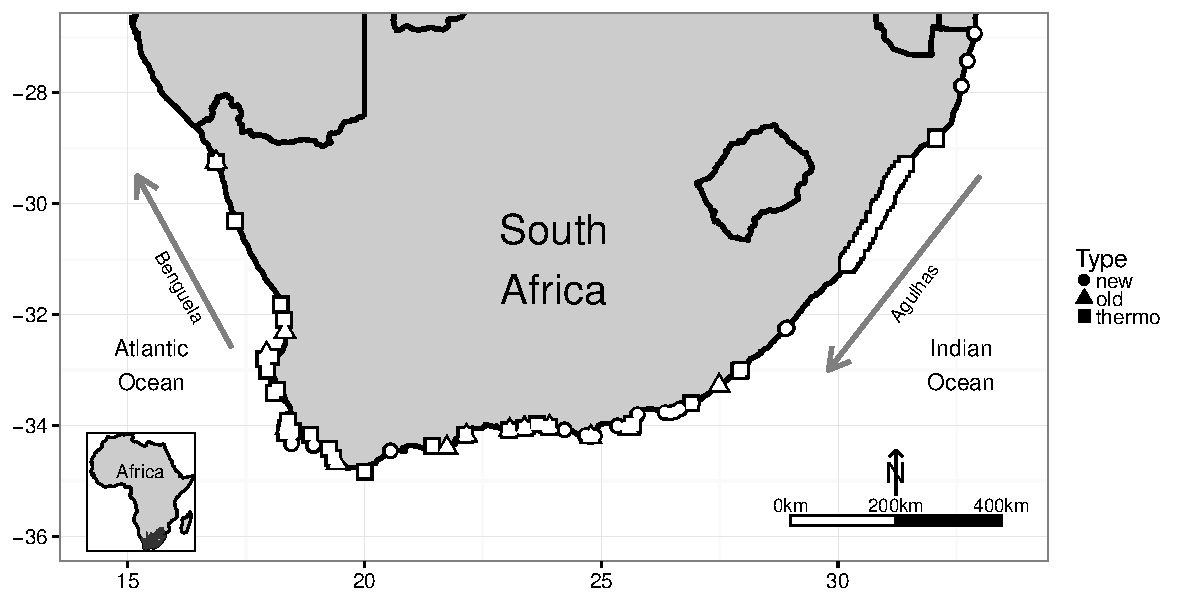
\includegraphics[width=1.0\textwidth]{figure01}
\caption{Map of South Africa indicating the location of the 129 time series comprising the South African Coastal Temperature Network. The location of the 84 time series used in this study are shown as solid white circles and the unused data sets as opaque.}
\label{figure01}
\end{figure}

\begin{figure}
\centering 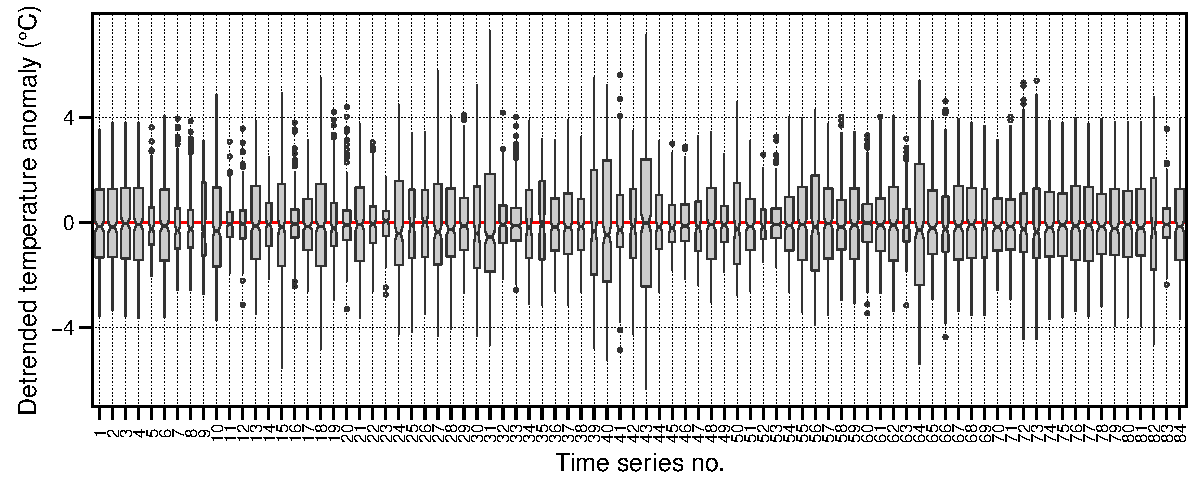
\includegraphics[width=1.0\textwidth]{figure02}
\caption{Box and whisker plot summarizing the 84 anomaly time series used in this study (\emph{i.e.} after detrending) but before adding a decadal trend or rounding the data. The plot indicates the first and third quartile as the extremities of the boxes, the median is shown as the horizontal line within each box, the minima and maxima are indicated by the whiskers and the points are outliers.}
\label{figure02}
\end{figure}

\begin{figure}
\centering 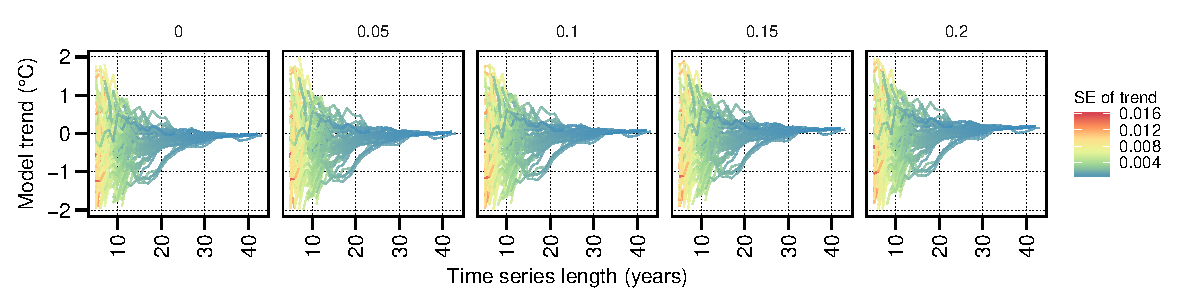
\includegraphics[width=1.0\textwidth]{figure03}
\caption{The effect of time series length on the ability of the GLS model to accurately detect the trend added to each time series. The box and whisker plot shows the first and third quartile as the extremities of the boxes, the median is shown as the horizontal line within each box, and the minima and maxima are indicated by the whiskers. Points indicate the spread of the actual data and their colors are scaled according to the length of the time series they represent.}
\label{figure03}
\end{figure}

\begin{figure}
\centering 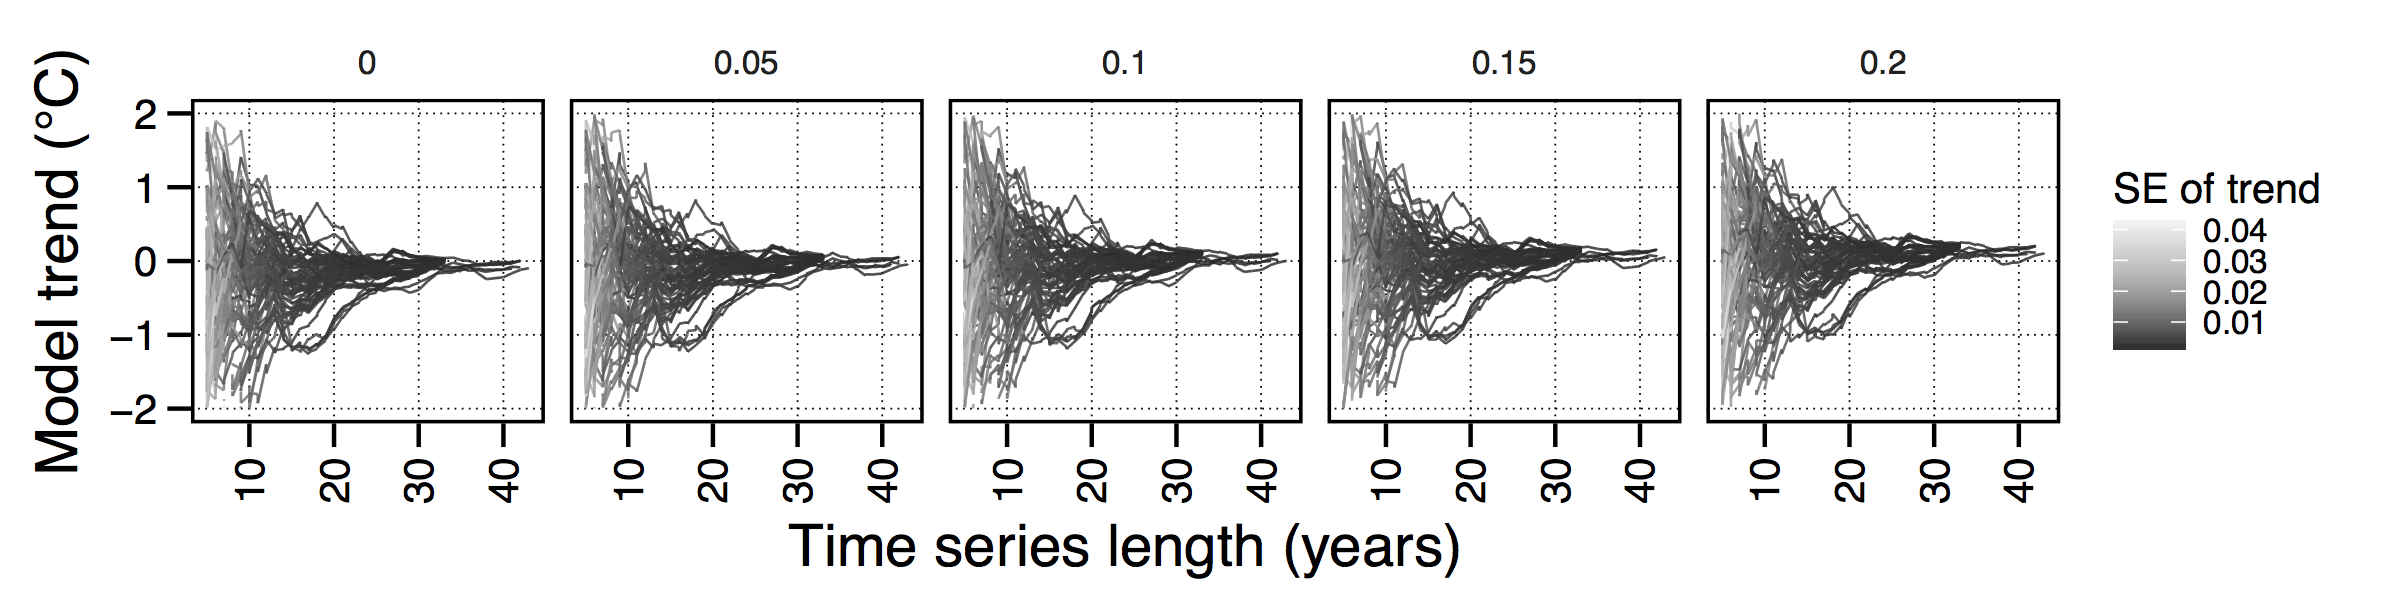
\includegraphics[width=1.0\textwidth]{figure04}
\caption{The relationship between the length of a time series, the size of the modeled trend and its standard error (SE). Each individual line shows the modeled trend for one of the 84 sites used in this analysis to which a model was fitted iteratively as the time series length was `grown' from 5 years in length to the maximum duration available for the site. The panels show the progressive effect that decadal trend has on this relationship (indicated by the numeral above each panel), and color is mapped to the SE of the trend.}
\label{figure04}
\end{figure}

\begin{figure}
\centering 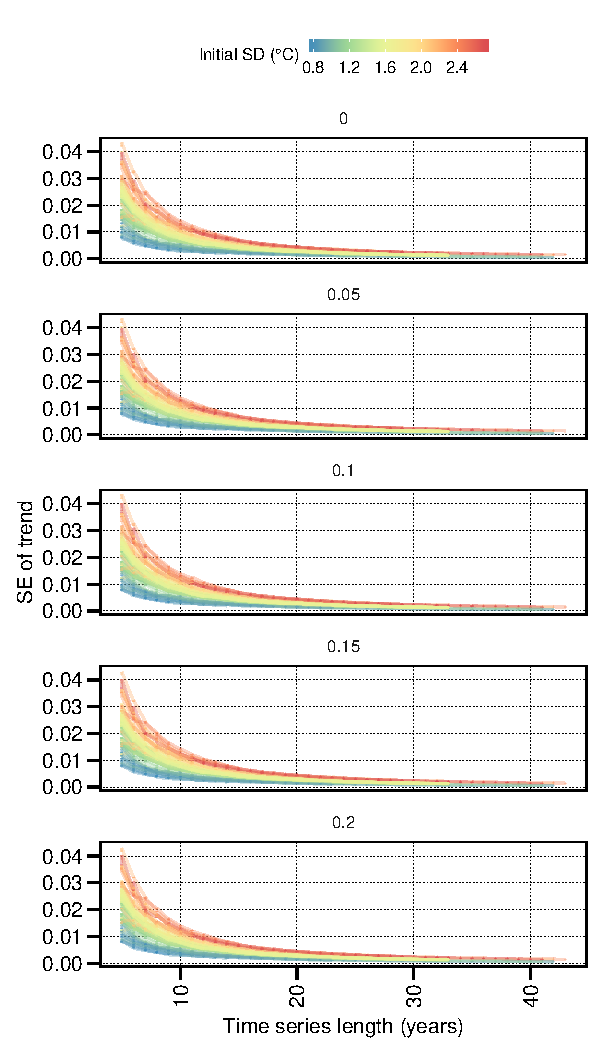
\includegraphics[width=0.65\textwidth]{figure05}
\caption{The effect of the SD of the anomaly time series before adding a decadal trend (`Initial SD'), or rounding the data to the different levels of precision, on the significance of the modeled trend. The size of the symbols are scaled in direct proportion to the time series length. Time series belonging to the three South African coastal sections are represented in color. The east coast (ec) typically has the most stable thermal regime of the three coasts, with the south coast (sc) having the greatest amount of variance and the west coast (wc) consisting of areas with both high and low variance. Linear models with 95\% confidence intervals (indicated by colored ribbons) have been fitted separately for each coastal section, and illustrate the interaction between Initial SD in each group and the significance (\emph{p}-value) of the GLS models. The panels, from top to bottom, show increasing decadal trends as indicated by numerals above the panels.}
\label{figure05}
\end{figure}

\begin{figure}
\centering 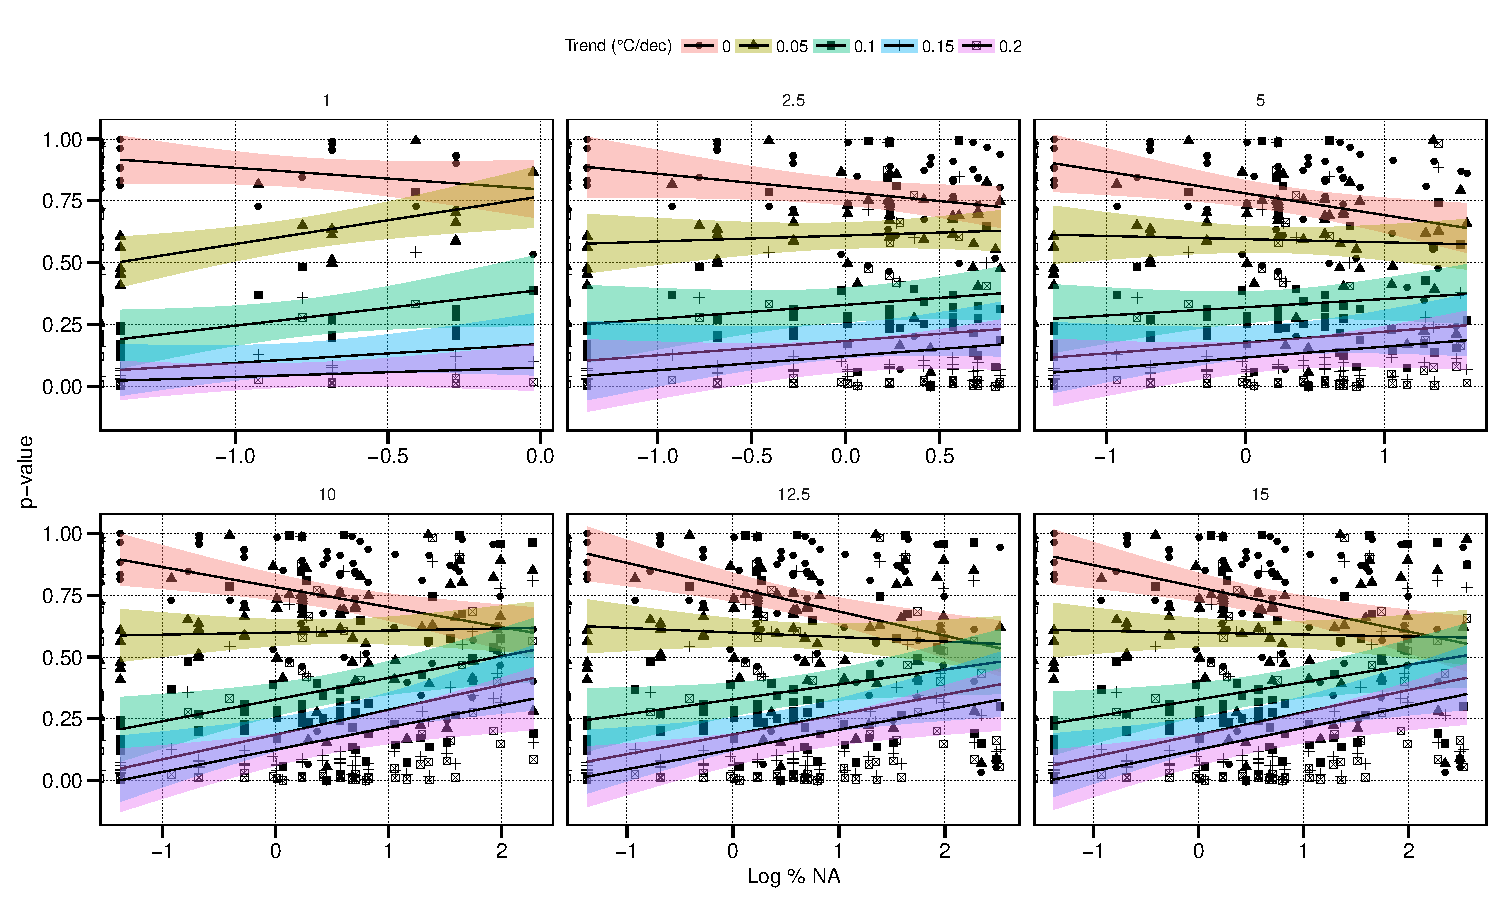
\includegraphics[width=0.65\textwidth]{figure06}
\caption{The relationship between the effect of Initial SD (\emph{i.e.} the variance of the anomaly time series before adding artificial decadal trends; shown here in color), on the standard error (SE) of a modeled trend, controlled for by the length of the time series. The effect of the size of the added decadal trends on the relationship is imperceptible and therefore only decadal trend of \SI{0.2}{\degreeCelsius}~dec$^{-1}$ is presented.}
\label{figure06}
\end{figure}

\begin{figure}
\centering 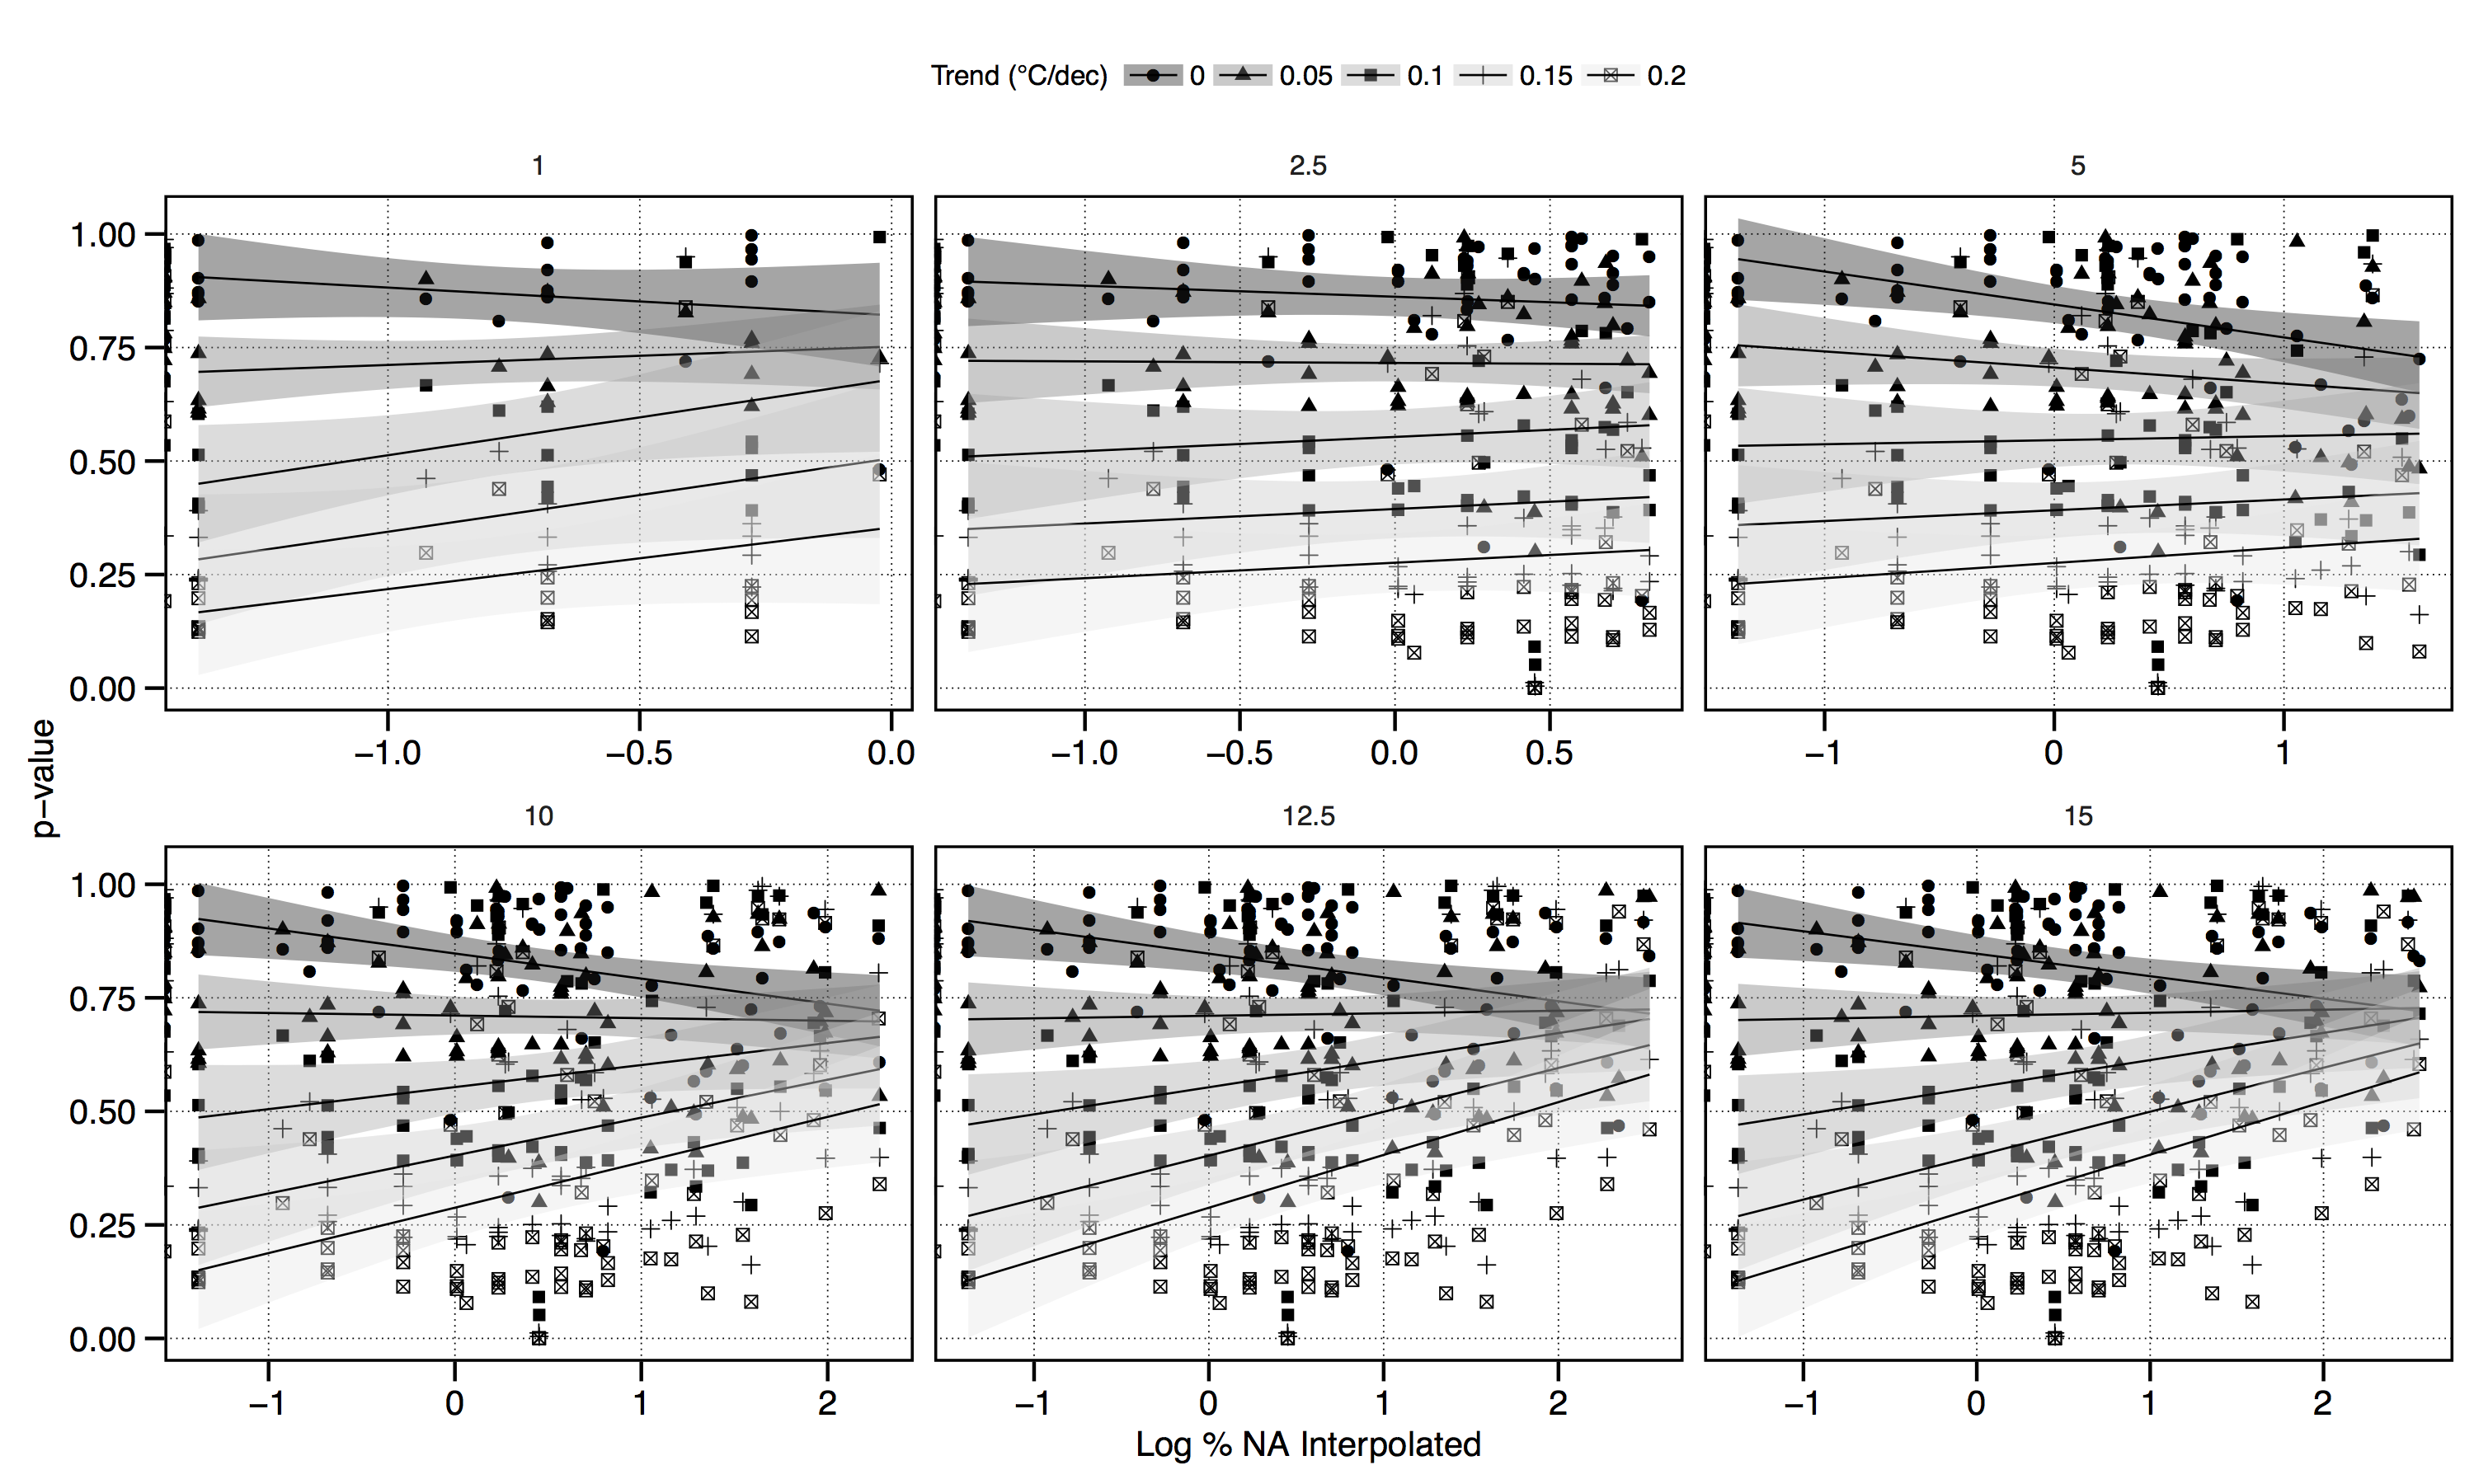
\includegraphics[width=1.0\textwidth]{figure07}
\caption{The relationship between the amount of missing values (\%\texttt{NA}) and the significance of a modeled trend. Each panel shows the effect of an increasingly larger amount of missing values, indicated above each panel by numerals. The fitted lines and 95\% confidence intervals (shown as colored bands) represent each of the five decadal trends assessed.}
\label{figure07}
\end{figure}

\begin{figure}
\centering 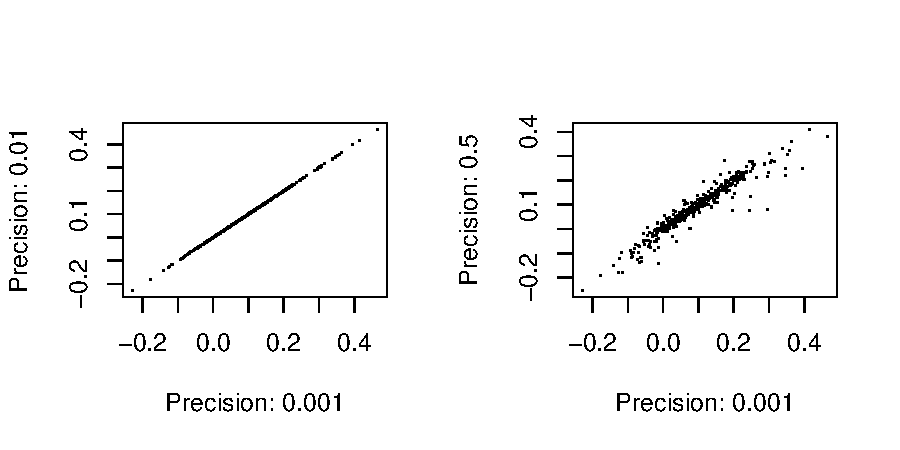
\includegraphics[width=1.0\textwidth]{figure08}
\caption{Plots representing correlations of the modeled trends acquired at different levels of rounding, which can be interpreted as representations of different measurement precisions. The effect of rounding from \SI{0.001}{\degreeCelsius} to \SI{0.01}{\degreeCelsius} may be seen in the panel on the left. The panel on the right shows that rounding from a precision of \SI{0.001}{\degreeCelsius} to \SI{0.5}{\degreeCelsius} has an visibly greater effect on the deterioration of the correlation between the two sets of estimated trends.}
\label{figure08}
\end{figure}

\end{document}